\documentclass[
    fontsize=12pt,          % default font size 12pt
    paper=a4,               % DIN A4 page format
    numbers=noenddot,       % remove dots behind chapter numbers (e.g. 1.5 not 1.5.)
    listof=totoc,           % add list of figures, tables, etc. to ToC
    listof=entryprefix,     % add entry name to figures, tables, etc.
    listof=nochaptergap,    % no chapter gap for figures, tables, etc.
    bibliography=totoc,     % add bibliography to ToC but without a chapter number
    parskip=half,           % half line spacing between paragraphs
    openany                 % chapters can start on any page
]{scrbook}

\include{../../for_latex/preamble}

\usepackage{amssymb}   % \checkmark

\begin{document}

    \begin{titlepage}
    	\pagestyle{empty}

    	% HFU Logo
    	\begin{flushright}
    		\begin{figure}[ht]
    			\flushright
    			
\includegraphics[height=2cm]{../../for_latex/hfu}
    		\end{figure}
    	\end{flushright}

    	\begin{center}
    		\vspace{3cm}

    		{\fontsize{22}{22} \selectfont \textbf{Blatt 7}}\\[5mm]
    		{\fontsize{18}{18} \selectfont Kryptologie}

    		\vspace{12cm}

    		{\fontsize{14}{14} \selectfont Luis Staudt}
    	\end{center}
    \end{titlepage}

% ############################################################################
% CONTENT STARTS HERE
% ############################################################################


\chapter*{Toy-Blockchain (SHA-256, Proof of Work)}


\section*{Aufgabenstellung}

Aufzubauen ist eine SHA-256-Blockchain der Länge~3, in der Rollen von Kunde und Miner
zusammenfallen.
Jeder Block enthält Transaktionsdaten, den Hash des Vorblocks (IV) und eine Nonce.
Der \emph{Proof of Work} verlangt, dass die führenden $k$ Nibbles \emph{aller drei}
Block-Hashes $0$ sind; dafür gibt es $k$ Punkte.

\begin{enumerate}[label=\alph*)]
    \item IV auf ALLZERO, Transaktionsnummer auf die Matrikelnummer setzen.
    \item Transaktionsdatenblock erzeugen (Felder (1)--(6)).
    \item Nonce so bestimmen, dass die führenden $k$ Nibbles des Hashes $0$ sind.
    \item Block um IV und Nonce ergänzen, Transaktionsnummer erhöhen, IV $:=$ Hash; zurück zu b).
    \item Blockchain in einem CrypTool2-Workspace nachstellen.
\end{enumerate}

\noindent\textbf{Ergebnis:} $k = 10$ führende Null-Nibbles in allen drei Blöcken.


\section*{Verwendete Werkzeuge}

\begin{itemize}
    \item \textbf{Eigener CUDA-Miner} (\texttt{miner.cu}) auf einer NVIDIA-GPU (entwickelt/getestet
          auf RTX~4070, Lauf auch auf RTX~4090) für das eigentliche Mining.
    \item \textbf{C-Referenz} (\texttt{reference.c}) mit identischer Nachrichten-Konstruktion zur
          unabhängigen Prüfung auf der CPU.
    \item \textbf{Python} (\texttt{hashlib}) als dritte, unabhängige SHA-256-Kontrolle.
    \item \textbf{CrypTool2} zum Nachbau der Blockchain (\texttt{Blockchain.cwm}).
\end{itemize}


\section*{Aufbau eines Blocks}

Gehasht wird die ASCII-Zeichenkette
\[
  \text{MESSAGE} \;=\; \text{IV} \,\Vert\, \text{TX} \,\Vert\, \text{\texttt{(8)}} \,\Vert\, \text{NONCE}
\]
mit den Bestandteilen:

\begin{itemize}
    \item \textbf{IV} (64 Hex): Block~1 $=$ ALLZERO ($64\times$\,\texttt{0}); danach jeweils der
          SHA-256-Hash des Vorblocks. Dies verkettet die Blöcke: $\text{IV}_n = H(\text{Block}_{n-1})$.
    \item \textbf{TX} (Transaktionsdaten):\\
          \texttt{(1)}\,Transaktionsnr (hex) \texttt{(2)}\,SHA1(Name)
          \texttt{(3)}\,Unixzeit \texttt{(4)}\,SHA1(Empfänger)
          \texttt{(5)}\,Betrag \texttt{(6)}\,Länge der Felder (1)--(5) \texttt{(7)}.
    \item \textbf{NONCE} (32 Hex, Feld \texttt{(8)}): der durch Mining gefundene Wert.
\end{itemize}

\noindent Die Transaktionsnummer startet bei der Matrikelnummer ($272056 = \texttt{0x426B8}$) und
wird je Block um~1 erhöht. Empfänger der drei Blöcke sind Alice, Bob und Carol.
Verwendete SHA1-Hashwerte:

\begin{lstlisting}[caption={SHA1 von Absender- und Empfängernamen}]
Name "Luis Noah Staudt" = D92AB98BB95D0DA30A4C9B38CBEC5F2642AA73F9
Alice                   = 35318264C9A98FAF79965C270AC80C5606774DF1
Bob                     = DA6645F6E22BF5F75974DC7EED5FCD6160D6B51E
Carol                   = 6F90F101115140727C43CADEE0B9E17881403A63
\end{lstlisting}


\section*{Mining (Proof of Work)}

SHA-256 ist eine kryptographische Hash-Funktion ohne Abkürzung: einen Hash mit $k$ führenden
Null-Nibbles findet man nur durch Ausprobieren. Da jede Nibble mit Wahrscheinlichkeit
$\tfrac{1}{16}$ null ist, trifft die Bedingung im Mittel jeden $16^{k}$-ten Versuch -- der Treffer
folgt einer geometrischen Verteilung mit Erwartungswert $16^{k}$ Hashes je Block.
Jede weitere Nibble kostet also den \textbf{16-fachen} Aufwand; das ist die Sicherheit des Proof
of Work. Für $k=10$ sind das $16^{10}\approx 1{,}1\cdot10^{12}$ Hashes je Block.

\subsection*{Optimierung: Midstate}

\textbf{Effizienz statt Trick.} Statt langsam in CrypTool2 zu minen, läuft die Suche offline auf der
GPU. SHA-256 verarbeitet die Nachricht in 512-Bit-Blöcken (je 64~Byte); pro Block läuft eine
Kompressionsfunktion. Beim Mining ändert sich von Versuch zu Versuch nur die Nonce ganz am Ende --
der gesamte Anfang (IV $+$ Transaktionsdaten) bleibt konstant. Diese konstanten Blöcke werden daher
\emph{einmalig} auf der CPU vorgehasht (\emph{Midstate}); die GPU lädt den Midstate, setzt nur den
variablen Zähler ein und rechnet pro Versuch lediglich die \emph{restlichen} Kompressionsschritte.

Konkret für Block~1 (analog für die anderen):

\begin{itemize}
    \item Nachricht $=$ IV $(64)$ $+$ TX $(121)$ $+$ \texttt{(8)} $+$ Nonce $(32)$ $=\;220$~Byte.
          Mit SHA-Padding ergibt das $\lceil(220+9)/64\rceil = \mathbf{4}$ Kompressionsblöcke.
    \item Konstanter Präfix (IV, TX, \texttt{(8)} und die 16~zufälligen High-Hexstellen der Nonce)
          $=204$~Byte $=$ \textbf{3 volle Blöcke}, die als Midstate vorgehasht werden.
    \item Die GPU variiert nur die 16~niederwertigen Hexstellen der Nonce und rechnet je Versuch
          \textbf{nur den letzten} der vier Blöcke -- ein Viertel der Arbeit pro Hash.
\end{itemize}

\noindent So erreicht die RTX~4070 einen Durchsatz von $\approx 3$\,GH/s. Bei $1{,}1\cdot10^{12}$
Hashes je Block liegt die \emph{erwartete} Suchzeit bei $\approx 6$~Minuten; wegen der geometrischen
Verteilung streuen die tatsächlichen Zeiten aber stark (Standardabweichung $\approx$ Erwartungswert):

\begin{table}[H]
    \centering
    \begin{tabular}{l l r}
        \toprule
        \textbf{Block} & \textbf{Empfänger} & \textbf{Suchzeit} \\
        \midrule
        1 & Alice & $1260$\,s $\;(\approx 21$\,min$)$ \\
        2 & Bob   & $\phantom{0}236$\,s $\;(\approx 4$\,min$)$ \\
        3 & Carol & $1091$\,s $\;(\approx 18$\,min$)$ \\
        \bottomrule
    \end{tabular}
    \caption{Gemessene Mining-Zeiten je Block bei $k=10$ (RTX~4090). Die große Streuung von
             $4$ bis $21$~Minuten entspricht der erwarteten geometrischen Verteilung.}
\end{table}

\noindent Damit liegt das erreichte $k=10$ deutlich über dem Musterbeispiel ($k=6$, $\approx 1{,}7\cdot10^7$
Hashes).


\section*{Ergebnis: Die drei Blöcke}

Gemeinsamer Zeitstempel (Feld (3)): Unixzeit \texttt{1781470311}.
Jeder Hash wurde unabhängig per \texttt{reference.c}, Python \texttt{hashlib} und CrypTool2
bestätigt; die Verkettung $\text{IV}_n = H(\text{Block}_{n-1})$ ist erfüllt.

\begin{lstlisting}[caption={Block 1 -- an Alice ($H$ mit 10 führenden Nullen)}]
IV   = 0000000000000000000000000000000000000000000000000000000000000000
TX   = (1)426B8(2)D92AB98BB95D0DA30A4C9B38CBEC5F2642AA73F9(3)1781470311
       (4)35318264C9A98FAF79965C270AC80C5606774DF1(5)42(6)112(7)
NONCE= (8)591b5f1056840691000000bc249430e6
HASH = 0000000000161F40BEAF0B2600EE1DD39E7B34F995702AD26F88E75A6053DE94
\end{lstlisting}

\begin{lstlisting}[caption={Block 2 -- an Bob}]
IV   = 0000000000161F40BEAF0B2600EE1DD39E7B34F995702AD26F88E75A6053DE94
TX   = (1)426B9(2)D92AB98BB95D0DA30A4C9B38CBEC5F2642AA73F9(3)1781470311
       (4)DA6645F6E22BF5F75974DC7EED5FCD6160D6B51E(5)100(6)113(7)
NONCE= (8)f4a8d8636e81d64d00000022ae2dcb1a
HASH = 00000000007BC41EE9F1021F56854A14CF2489DD793EC8C0CE8F360185AF6BA2
\end{lstlisting}

\begin{lstlisting}[caption={Block 3 -- an Carol}]
IV   = 00000000007BC41EE9F1021F56854A14CF2489DD793EC8C0CE8F360185AF6BA2
TX   = (1)426BA(2)D92AB98BB95D0DA30A4C9B38CBEC5F2642AA73F9(3)1781470311
       (4)6F90F101115140727C43CADEE0B9E17881403A63(5)7(6)111(7)
NONCE= (8)53da94499e68bd340000009f34dc1743
HASH = 00000000004BB8BD740A25D5B36C419B7668DBC34DC73352264D00C606466331
\end{lstlisting}

\noindent\emph{Hinweis:} In den TX-Strings ist der Zeilenumbruch vor \texttt{(4)} nur durch die
Spaltenbreite bedingt; gehasht wird die ununterbrochene Zeichenkette.


\section*{Verifikation}

Die SHA-256-Implementierung wird zunächst gegen den offiziellen Testvektor geprüft
(\texttt{reference.c}, Selbsttest beim Start):

\begin{lstlisting}[caption={Selbsttest gegen den bekannten SHA-256-Testvektor}]
SHA256("abc") = BA7816BF8F01CFEA414140DE5DAE2223B00361A396177A9CB410FF61F20015AD
expected      = BA7816BF8F01CFEA414140DE5DAE2223B00361A396177A9CB410FF61F20015AD   [OK]
\end{lstlisting}

\noindent Anschließend wird jeder Block-Hash mit einer dritten, völlig unabhängigen
Implementierung -- Pythons \texttt{hashlib} -- nachgerechnet, z.\,B. für Block~1:

\begin{lstlisting}[language=Python, caption={Unabhängige Kontrolle mit Python \texttt{hashlib} (Block 1)}]
$ python3 -c "import hashlib; \
  iv='0'*64; \
  tx='(1)426B8(2)D92AB98BB95D0DA30A4C9B38CBEC5F2642AA73F9(3)1781470311' \
     '(4)35318264C9A98FAF79965C270AC80C5606774DF1(5)42(6)112(7)'; \
  nonce='(8)591b5f1056840691000000bc249430e6'; \
  print(hashlib.sha256((iv+tx+nonce).encode()).hexdigest())"
0000000000161f40beaf0b2600ee1dd39e7b34f995702ad26f88e75a6053de94
\end{lstlisting}

\noindent Alle drei Implementierungen (CUDA, C, Python) und CrypTool2 liefern für jeden Block
denselben Hash; die zehn führenden Null-Nibbles sind reproduzierbar bestätigt.


\section*{Nachbau in CrypTool2}

Der Workspace \texttt{Blockchain.cwm} bildet die Kette je Block mit
\texttt{Text Input} $\rightarrow$ \texttt{Concatenate} $\rightarrow$ \texttt{SHA-256}
$\rightarrow$ \texttt{Text Output} nach:

\begin{enumerate}
    \item Drei \texttt{Text Input}: IV (64 Hex), TX-String, \texttt{(8)}$+$NONCE.
    \item Mit \texttt{Concatenate} in der Reihenfolge IV~$\Vert$~TX~$\Vert$~Nonce zusammenfügen.
    \item In \texttt{SHA-256} geben; das \texttt{Text Output} zeigt den Hash mit zehn führenden
          Nullen.
    \item Der Output-Hash von Block~$n$ ist die IV-Eingabe von Block~$n{+}1$ (Kette).
\end{enumerate}

\begin{figure}[H]
    \centering
    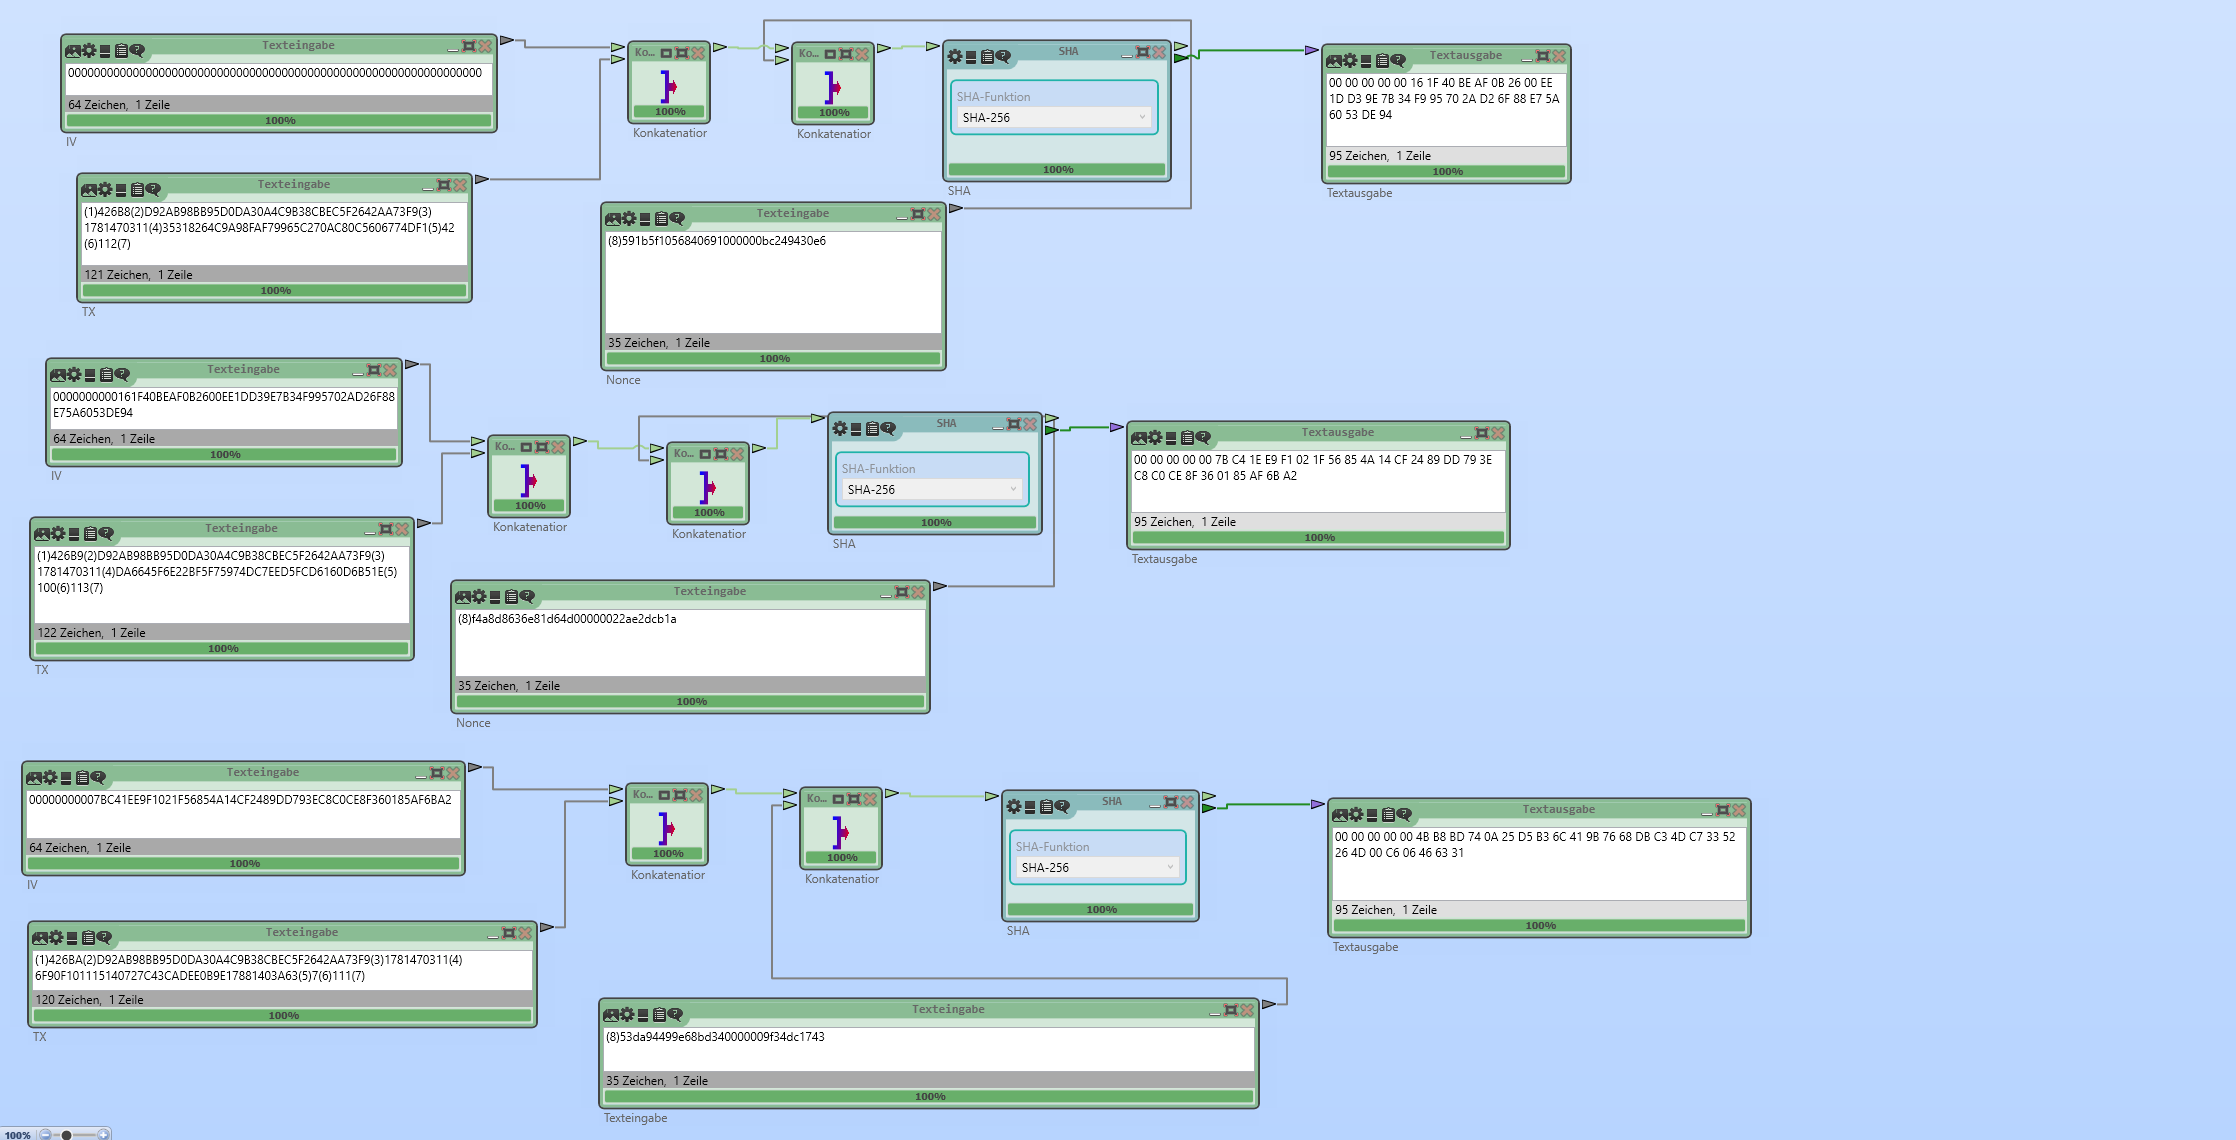
\includegraphics[width=\linewidth]{Blockchain}
    \caption{CrypTool2-Workspace (\texttt{Blockchain.cwm}): die drei verketteten Blöcke. Jeder
             \texttt{Texteingabe}-Strang (IV, TX, Nonce) wird per \texttt{Konkatenation} zusammengeführt
             und in \texttt{SHA-256} gehasht. Die \texttt{Textausgabe} jedes Blocks zeigt den Hash mit
             zehn führenden Null-Nibbles (\texttt{00 00 00 00 00 \dots}) und dient zugleich als
             IV-Eingabe des nächsten Blocks -- die Verkettung ist damit sichtbar erfüllt.}
\end{figure}


\section*{Bewertung}

\begin{itemize}
    \item Alle drei Block-Hashes erfüllen die Anforderung mit $\mathbf{k=10}$ führenden
          Null-Nibbles; die Verkettung über den IV ist lückenlos.
    \item SHA-256 lässt sich nicht ``austricksen'' -- der einzige Hebel ist roher Durchsatz.
          Der Midstate-Trick (konstante Blöcke vorhashen) und die GPU bringen $k$ klar über das
          Musterbeispiel.
    \item Drei unabhängige SHA-256-Implementierungen (CUDA, C, Python) sowie CrypTool2 liefern
          identische Hashes -- die Lösung ist reproduzierbar verifiziert.
\end{itemize}

% ############################################################################
% CONTENT ENDS HERE
% ############################################################################

\end{document}
